\section{The SIR Model}
To explain the concepts of ABS and of our functional reactive approach to it, we introduce the SIR model as a motivating example. It is a very well studied and understood compartment model from epidemiology \cite{kermack_contribution_1927} which allows to simulate the dynamics of an infectious disease like influenza, tuberculosis, chicken pox, rubella and measles \cite{enns_its_2010} spreading through a population. In this model, people in a population of size $N$ can be in either one of three states \textit{Susceptible}, \textit{Infected} or \textit{Recovered} at a particular time, where it is assumed that initially there is at least one infected person in the population. People interact with each other \textit{on average} with a given rate $\beta$ per time-unit and get infected with a given probability $\gamma$ when interacting with an infected person. When infected, a person recovers \textit{on average} after $\delta$ time-units and is then immune to further infections. An interaction between infected persons does not lead to re-infection, thus these interactions are ignored in this model. This definition gives rise to three compartments with the transitions as seen in Figure \ref{fig:sir_transitions}.

\begin{figure}
	\centering
	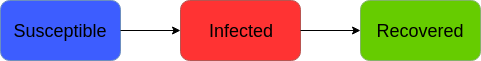
\includegraphics[width=.4\textwidth, angle=0]{./../shared/fig/diagrams/SIR_transitions.png}
	\caption{Transitions in the SIR compartment model.}
	\label{fig:sir_transitions}
\end{figure}

The dynamics of this model over time can be formalized using the System Dynamics (SD) approach \cite{porter_industrial_1962} which models a system through differential equations. For the SIR model we get the following equations:

\begin{align}
\frac{\mathrm d S}{\mathrm d t} &= -infectionRate \\ 
\frac{\mathrm d I}{\mathrm d t} &= infectionRate - recoveryRate \\ 
\frac{\mathrm d R}{\mathrm d t} &= recoveryRate 
\end{align}

\begin{align}
infectionRate &= \frac{I \beta S \gamma}{N} \\
recoveryRate &= \frac{I}{\delta} 
\end{align}

Solving these equations is then done by integrating over time. In the SD terminology, the integrals are called \textit{Stocks} and the values over which is integrated over time are called \textit{Flows}. The $1+$ in $I(t)$ amounts to the initially infected agent - if there wouldn't be a single infected one, the system would immediately reach equilibrium.

\begin{align}
S(t) &= N + \int_0^t -infectionRate\, \mathrm{d}t \\
I(t) &= 1 + \int_0^t infectionRate - recoveryRate\, \mathrm{d}t \\
R(t) &= \int_0^t recoveryRate\, \mathrm{d}t
\end{align}

There exist a huge number of software packages which allow to conveniently express SD models using a visual approach like in Figure \ref{fig:sir_sd_stockflow_diagramm}.

\begin{figure}
	\centering
	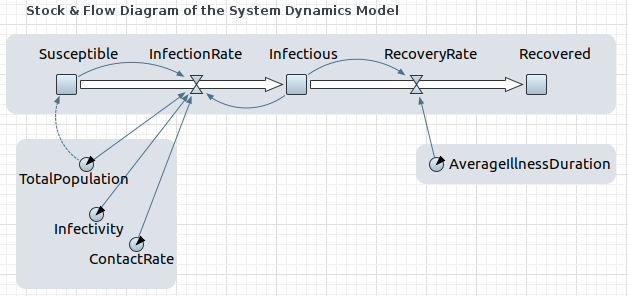
\includegraphics[width=.4\textwidth, angle=0]{./../shared/fig/diagrams/SIR_SD_STOCKFLOW_DIAGRAMM.png}
	\caption{A visual representation of the SD stocks and flows of the SIR compartment model. Picture taken using AnyLogic Personal Learning Edition 8.1.0.}
	\label{fig:sir_sd_stockflow_diagramm}
\end{figure}

Running the SD simulation over time results in the dynamics as shown in Figure \ref{fig:sir_sd_dynamics} with the given variables.

\begin{figure}
	\centering
	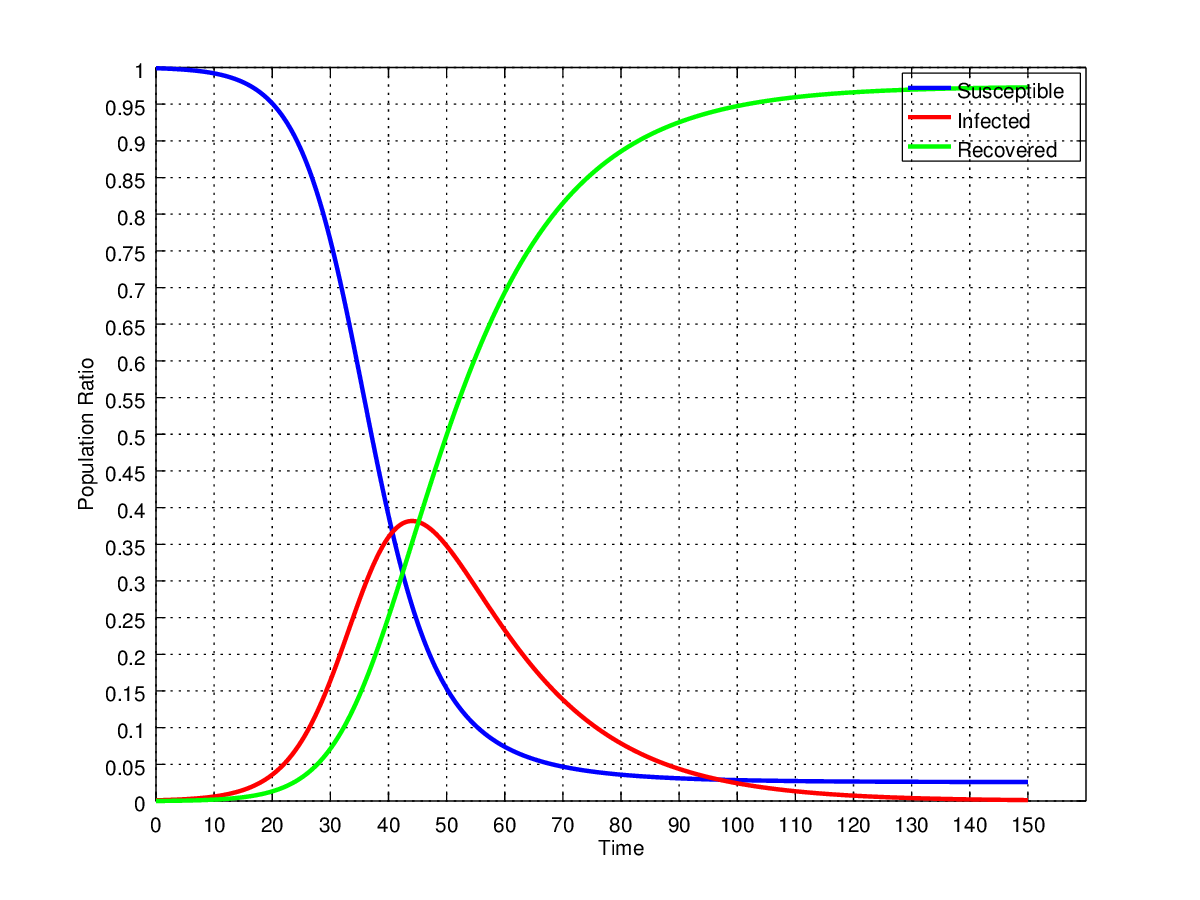
\includegraphics[width=.4\textwidth, angle=0]{./../shared/fig/frsd/SIR_SD_1000agents_150t_001dt.png}
	\caption{Dynamics of the SIR compartment model using the System Dynamics approach. Population Size $N$ = 1,000, contact rate $\beta =  \frac{1}{5}$, infection probability $\gamma = 0.05$, illness duration $\delta = 15$ with initially 1 infected agent. Simulation run for 150 time-steps.}
	\label{fig:sir_sd_dynamics}
\end{figure}

\subsection*{An Agent-Based approach}
The SD approach is inherently top-down because the emergent property of the system is formalized in differential equations. The question is if such a top-down behaviour can be emulated using ABS, which is inherently bottom-up. Also the question is if there are fundamental drawbacks and benefits when doing so using ABS. Such questions were asked before and modelling the SIR model using an agent-based approach is indeed possible. It is important to note that SD can be seen as operating on averages thus treating the population completely continuous which results in non-discrete values of stocks e.g. 3.1415 infected persons. Thus the fundamental approach to map the SIR model to an ABS is to discretize the population and model each person in the population as an individual agent. The transition  between the states are no longer happening according to continuous differential equations but due to discrete events caused both by interactions amongst the agents and time-outs.

TODO: this is already a too technical explanation which fixes the implementation details already on messaging / data-flow - this is too early and in deriving our approach we will implement 4 different approaches (feedback of all agent-states, data-flow, environment, transactions)
TODO: the main point is that we are implementing a state-chart with the transitions are the main thing to consider

\begin{itemize}
	\item Every agent makes \textit{on average} contact with $\beta$ random other agents per time unit. In ABS we can only contact discrete agents thus we model this by generating a random event on average every $\beta$ time units. Note that we need to sample from an exponential CDF because the rate is proportional to the size of the population as \cite{borshchev_system_2004} pointed out.
	
	\item An agent does not know the other agents' state when making contact with it, thus we need a mechanism in which agents reveal their state in which they are in \textit{at the moment of making contact}. Obviously the already mentioned messaging which allows agents to interact is perfectly suited to do this.
	\begin{itemize}
		\item \textit{Susceptibles}: These agents make contact with other random agents (excluding themselves) with a "Susceptible" message. They can be seen to be the drivers of the dynamics.
		\item \textit{Infected}: These agents only reply to incoming "Susceptible" messages with an "Infected" message to the sender. Note that they themselves do \textit{not} make contact pro-actively but only react to incoming one. 
		\item \textit{Recovered}: These agents do not need to send messages because contacting it or being contacted by it has no influence on the state.
	\end{itemize}
	
	\item Transition of susceptible to infected state - a susceptible agent needs to have made contact with an infected agent which happens when it receives an "Infected" message. If this happens an infection occurs with a probability of $\gamma$. The infection can be calculated by drawing $p$ from a uniform random-distribution between 0 and 1 - infection occurs in case of $\gamma >= p $. Note that this needs to be done for \textit{every} received "Infected" message.
	
	\item Transition of infected to recovered - a person recovers \textit{on average} after $\delta$ time unites. This is implemented by drawing the duration from an exponential distribution \cite{borshchev_system_2004} with $\lambda = \frac{1}{\delta}$ and making the transition after this duration.
\end{itemize}

For a more in-depth introduction of how to approximate an SD model by ABS see \cite{macal_agent-based_2010} who discusses a general approach and how to compare dynamics and \cite{borshchev_system_2004} which explain the need to draw the illness-duration from an exponential-distribution. For comparing the dynamics of the SD and ABS approach to real-world epidemics see \cite{ahmed_variance_2013}.